\documentclass[tikz,border=8pt]{standalone}
\usepackage{amsmath,amssymb}
\begin{document}
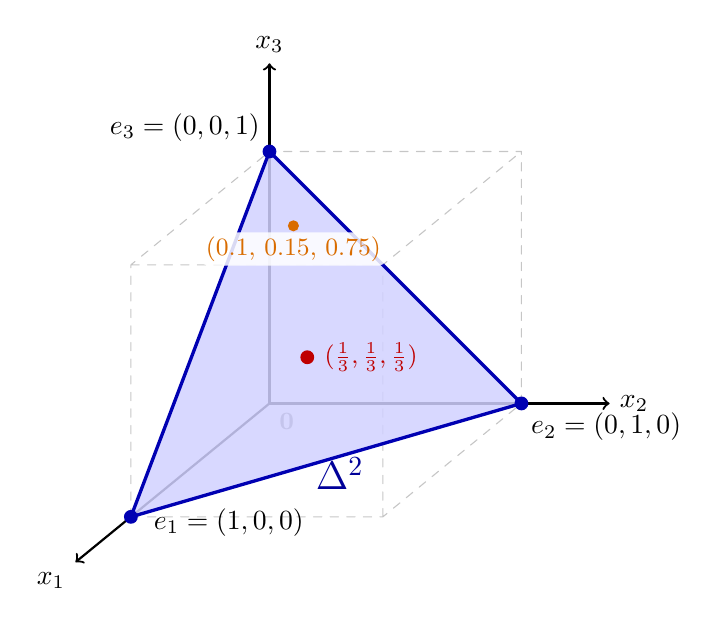
\begin{tikzpicture}[
    x={(-0.55cm,-0.45cm)}, y={(1cm,0cm)}, z={(0cm,1cm)},
    scale=3.2, line join=round, line cap=round,
    dot/.style={circle, fill, inner sep=0pt, minimum size=#1},
    dot/.default=5pt]
  % Cubo unitario (referencia)
  \draw[gray!45, dashed, thin]
    (1,0,0)--(1,1,0)--(0,1,0)  (1,0,0)--(1,0,1)--(0,0,1)
    (0,1,0)--(0,1,1)--(0,0,1)  (1,1,0)--(1,1,1)
    (1,0,1)--(1,1,1)--(0,1,1);
  % Ejes
  \draw[->, thick] (0,0,0) -- (1.4,0,0) node[anchor=north east] {$x_1$};
  \draw[->, thick] (0,0,0) -- (0,1.35,0) node[anchor=west] {$x_2$};
  \draw[->, thick] (0,0,0) -- (0,0,1.35) node[anchor=south] {$x_3$};
  \node[anchor=north west, font=\small, gray] at (0,0,0) {$\mathbf{0}$};
  % Símplex
  \filldraw[fill=blue!18, fill opacity=0.85, draw=blue!70!black, very thick]
    (1,0,0) -- (0,1,0) -- (0,0,1) -- cycle;
  % Vértices (one-hot)
  \node[dot, blue!70!black] at (1,0,0) {};
  \node[anchor=west] at (1.05,0.08,0) {$e_1=(1,0,0)$};
  \node[dot, blue!70!black] at (0,1,0) {};
  \node[anchor=north west] at (0,1,0) {$e_2=(0,1,0)$};
  \node[dot, blue!70!black] at (0,0,1) {};
  \node[anchor=south east] at (0,0,1) {$e_3=(0,0,1)$};
  % Centro (distribución uniforme)
  \node[dot, red!75!black] (c) at (1/3,1/3,1/3) {};
  \node[anchor=west, font=\small, red!75!black] at (c.east)
    {$(\tfrac13,\tfrac13,\tfrac13)$};
  % Punto suave cercano a e3
  \node[dot=4pt, orange!85!black] (p) at (0.1,0.15,0.75) {};
  \node[anchor=north, font=\small, orange!85!black, fill=white, fill opacity=0.85, text opacity=1, inner sep=1.5pt, rounded corners=2pt] at (p.south)
    {$(0.1,\,0.15,\,0.75)$};
  % Etiqueta
  \node[font=\Large, blue!60!black] at (0.62,0.62,0.0) {$\Delta^2$};
\end{tikzpicture}
\end{document}
